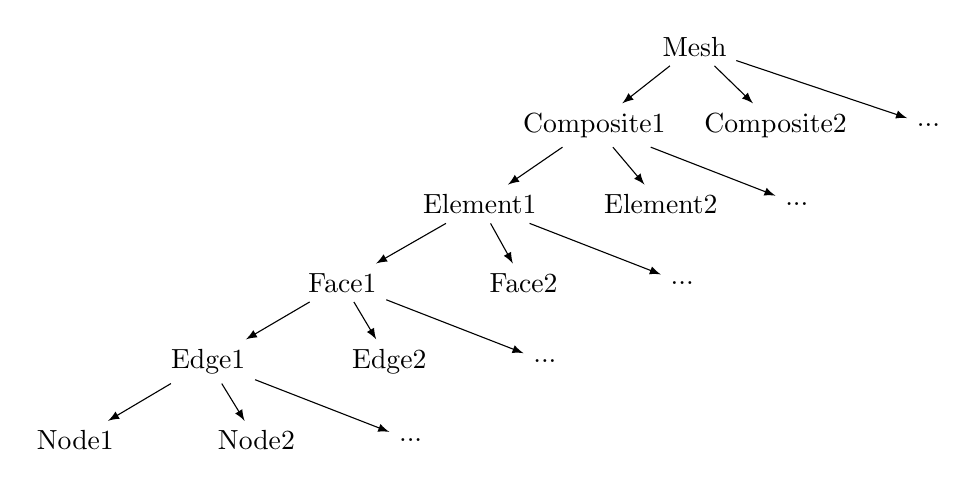
\begin{tikzpicture}[
  sibling distance=23mm, 
  level distance=10mm,
  edge from parent/.style={draw,-latex}, 
  grow=south,
  every node/.style={anchor=west}
]

% Root node
\node {Mesh}
  child {node {Composite1}
    child {node {Element1}
      child {node {Face1}
        child {node {Edge1}
          child {node {Node1}}
          child {node {Node2}}
          child {node {...}}}
        child {node {Edge2}}
        child {node {...}}}
      child {node {Face2}}
      child {node {...}}}
    child {node {Element2}}
    child {node {...}}}
  child {node {Composite2}}
  child [sibling distance=27mm]{node {...}};

\end{tikzpicture}